% Tikz File 'model640.tex'
\documentclass{standalone}
\usepackage{tikz} %Graphics
\usepackage{pgfplots} % XY plots

%\usetikzlibrary{...}
\begin{document}
	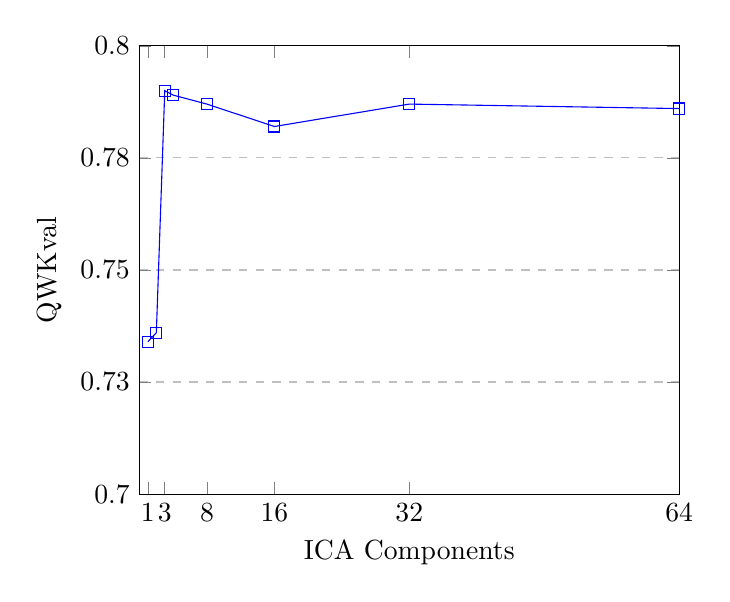
\begin{tikzpicture}
		\begin{axis}[
		%title={Receptive field vs Layer},
		xlabel={ICA Components},
		ylabel={QWKval},
		xmin=0, xmax=64,
		ymin=0.700, ymax=0.800,
		xtick={1,3,8,16,32,64},
		ytick={0.700, 0.725, 0.750, 0.775, 0.800},
		legend pos=north west,
		ymajorgrids=true,
		grid style=dashed,
		]
		
		\addplot[
		color=blue,
		mark=square,
		]
		coordinates {
			(1,0.734)(2,0.736)(3,0.790)(4,0.789)(8,0.787)(16,0.782)(32,0.787)(64,0.786)
		};
		%\legend{CuSO$_4\cdot$5H$_2$O}
		
		\end{axis}
	\end{tikzpicture}
\end{document}
